%%%%%%%%%%%%%%%%%%%%%%%%%%%%%%%%%%%%%%%%%
% Stylish Article
% LaTeX Template
% Version 2.1 (1/10/15)
%
% This template has been downloaded from:
% http://www.LaTeXTemplates.com
%
% Original author:
% Mathias Legrand (legrand.mathias@gmail.com) 
% With extensive modifications by:
% Vel (vel@latextemplates.com)
%
% License:
% CC BY-NC-SA 3.0 (http://creativecommons.org/licenses/by-nc-sa/3.0/)
%
%%%%%%%%%%%%%%%%%%%%%%%%%%%%%%%%%%%%%%%%%

%----------------------------------------------------------------------------------------
%	PACKAGES AND OTHER DOCUMENT CONFIGURATIONS
%----------------------------------------------------------------------------------------

\documentclass[fleqn,12pt]{SelfArx} % Document font size and equations flushed left

% \usepackage[english]{babel} % Specify a different language here - english by default

\usepackage[T1]{fontenc}
\usepackage[brazil]{babel}
\usepackage[brazil]{varioref}
\usepackage[utf8]{inputenc}

\usepackage{lipsum} % Required to insert dummy text. To be removed otherwise

%----------------------------------------------------------------------------------------
%	COLUMNS
%----------------------------------------------------------------------------------------

\setlength{\columnsep}{0.55cm} % Distance between the two columns of text
\setlength{\fboxrule}{0.75pt} % Width of the border around the abstract

%----------------------------------------------------------------------------------------
%	COLORS
%----------------------------------------------------------------------------------------

\definecolor{color1}{RGB}{0,0,90} % Color of the article title and sections
\definecolor{color2}{RGB}{0,20,20} % Color of the boxes behind the abstract and headings

%----------------------------------------------------------------------------------------
%	HYPERLINKS
%----------------------------------------------------------------------------------------

\usepackage{hyperref} % Required for hyperlinks

\hypersetup{hidelinks,
            colorlinks,
            breaklinks=true,
            urlcolor=color2,
            citecolor=color1,
            linkcolor=color1,
            bookmarksopen=false,
            pdftitle={Title},
            pdfauthor={Author}
            }

\usepackage[autostyle]{csquotes}
\usepackage[backend=biber]{biblatex}

\addbibresource{sample.bib}

%----------------------------------------------------------------------------------------
%	ARTICLE INFORMATION
%----------------------------------------------------------------------------------------

\JournalInfo{UFRPE, 13/08/2018}
\Archive{Disciplina de computação evolutiva}

\PaperTitle{
União de métodos de processamentos de imagens digitais, que encadeado em
processo de reconhecimento dígitos escritos a mão livre
} % Article title

\Authors{Iury Adones Xavier dos Santos\textsuperscript{1}*,
         Dr. Adenilton Jos\'{e} da Silva\textsuperscript{2},
         Dr. P\'{e}ricles Barbosa Cunha de Miranda\textsuperscript{3},
         Dr. Danilo Ricardo Barbosa de Araújo\textsuperscript{4},
         } % Authors

\affiliation{
\textsuperscript{1}\textit{Programa de Pós-Graduação em Informatica Aplicada (PPGIA), Universidade Federal Rural de Pernambuco (UFRPE), Recife-PE, Brasil}
} % Author affiliation

\affiliation{*\textbf{Autor correspondente}: iuryadones@gmail.com} % Corresponding author

\Keywords{
Algoritmos genéticos --- Processamento encadeado --- Reconhecimento de dígitos 
} % Keywords - if you don't want any simply remove all the text between the curly brackets

\newcommand{\keywordname}{Palavras-chaves} % Defines the keywords heading name

%----------------------------------------------------------------------------------------
%	ABSTRACT
%----------------------------------------------------------------------------------------

\Abstract{
Neste presente trabalho, têm experimentos voltados na área de processamento de
imagens digitais e heurística voltada ao reconhecimento de números escritos, no
entanto, aborda-se alguns passos antes mesmo de chegar-se ao reconhecimento dos
dígitos. Nesses passos que nos revela um fluxo encadeado, são atualmente
produzidos nas literaturas acadêmicas as seções do fluxo de processamento de
imagens, que inicia desda aquisição da imagem bruta, limpeza de ruídos e
binarização dos objetos, pode compor até mesmo com reconhecimento de objetos.
Tais trechos da trajetória do encadeamento, necessita de métodos de otimização,
pois melhoram os resultados, tanto na visualização e classificação. Nós
construirmos experimentos, que testa algumas das possíveis combinações dos
fluxos de encadeamento, estão contidas em um espaço de busca restrito, e nesta
construção abordamos com métodos baseado em algoritmos genéticos, que nos
informa quais as melhores combinações do fluxo encadeado, passadas por avaliação
de minimização do quantitativo de erros na detecção dos dígitos, sem a
necessidade de otimizar cada seção por vez.
}

%----------------------------------------------------------------------------------------

\begin{document}

\flushbottom % Makes all text pages the same height

\maketitle % Print the title and abstract box

\tableofcontents % Print the contents section

\thispagestyle{empty} % Removes page numbering from the first page

%----------------------------------------------------------------------------------------
%	ARTICLE CONTENTS
%----------------------------------------------------------------------------------------

\medskip

\section*{Introdução} % The \section*{} command stops section numbering

\addcontentsline{toc}{section}{Introdução} % Adds this section to the table of contents

\lipsum[1] % Dummy text
 and some mathematics $\cos\pi=-1$ and $\alpha$ in the text\footnote{And some
 mathematics $\cos\pi=-1$ and $\alpha$ in the text.}.

%------------------------------------------------

\section{Metodologia}

\begin{figure*}[ht]\centering % Using \begin{figure*} makes the figure take up the entire width of the page
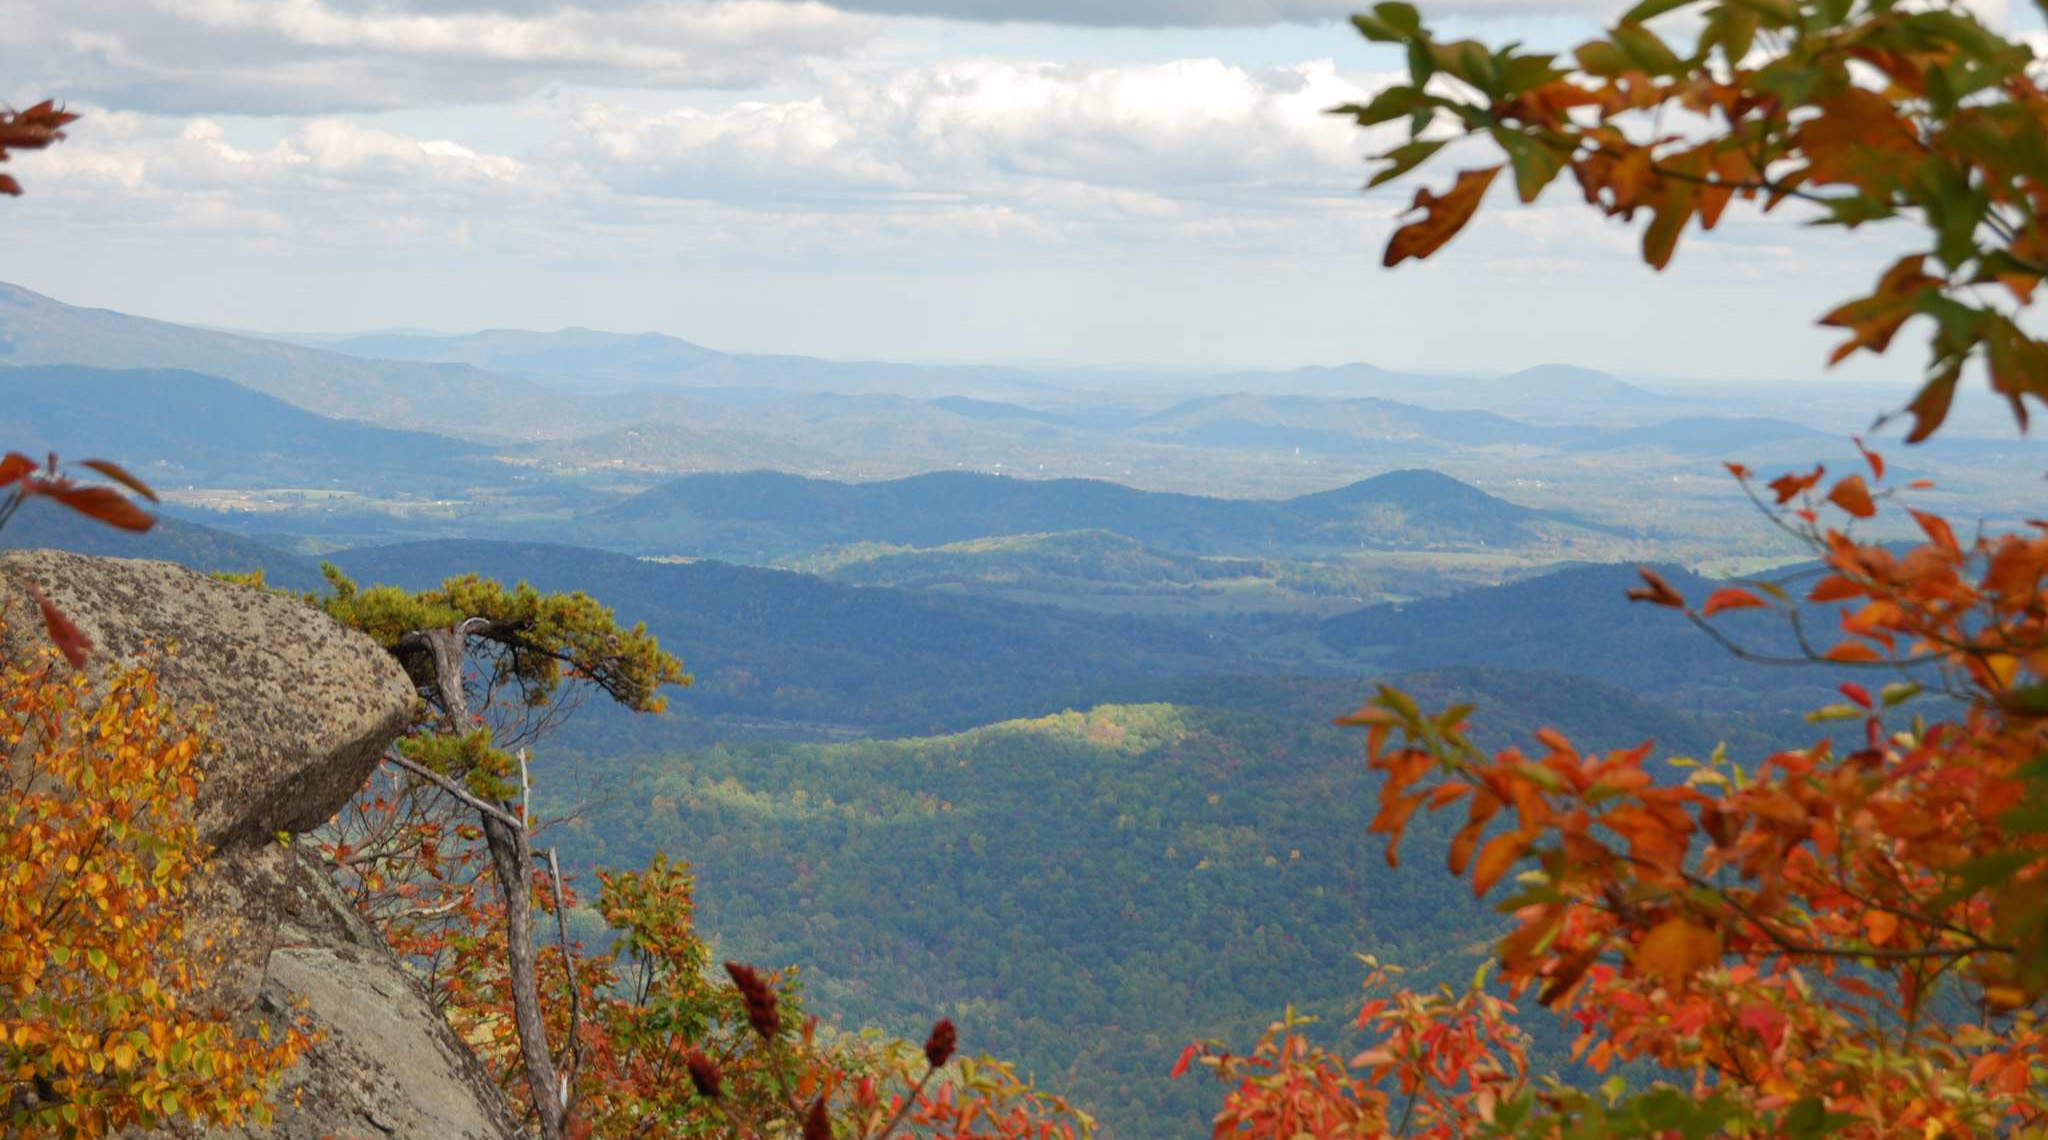
\includegraphics[width=\linewidth]{view}
\caption{Wide Picture}
\label{fig:view}
\end{figure*}

\lipsum[4] % Dummy text

\begin{equation}
\cos^3 \theta =\frac{1}{4}\cos\theta+\frac{3}{4}\cos 3\theta
\label{eq:refname2}
\end{equation}

\lipsum[5] % Dummy text

\begin{enumerate}[noitemsep] % [noitemsep] removes whitespace between the items for a compact look
\item First item in a list
\item Second item in a list
\item Third item in a list
\end{enumerate}

\subsection{Subsection}

\lipsum[6] % Dummy text

\paragraph{Paragraph} \lipsum[7] % Dummy text
\paragraph{Paragraph} \lipsum[8] % Dummy text

\subsection{Subsection}

\lipsum[9] % Dummy text

\begin{figure}[ht]\centering
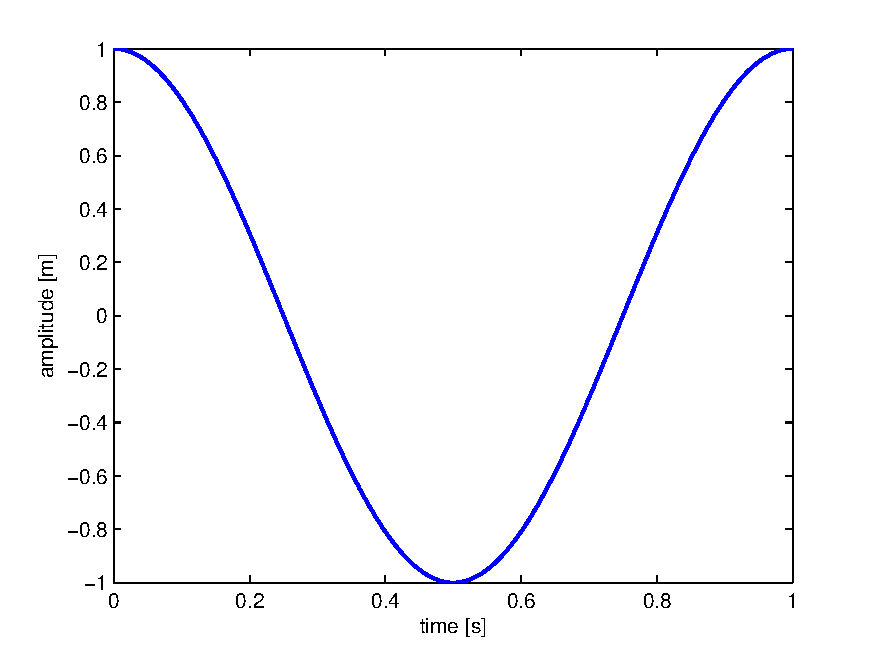
\includegraphics[width=\linewidth]{results}
\caption{In-text Picture}
\label{fig:results}
\end{figure}

Reference to Figure \ref{fig:results}.

%------------------------------------------------

\section{Results and Discussion}

\lipsum[10] % Dummy text

\subsection{Subsection}

\lipsum[11] % Dummy text

\begin{table}[hbt]
\caption{Table of Grades}
\centering
\begin{tabular}{llr}
\toprule
\multicolumn{2}{c}{Name} \\
\cmidrule(r){1-2}
First name & Last Name & Grade \\
\midrule
John & Doe & $7.5$ \\
Richard & Miles & $2$ \\
\bottomrule
\end{tabular}
\label{tab:label}
\end{table}

\subsubsection{Subsubsection}

\lipsum[12] % Dummy text

\begin{description}
\item[Word] Definition
\item[Concept] Explanation
\item[Idea] Text
\end{description}

\subsubsection{Subsubsection}

\lipsum[13] % Dummy text

\begin{itemize}[noitemsep] % [noitemsep] removes whitespace between the items for a compact look
\item First item in a list
\item Second item in a list
\item Third item in a list
\end{itemize}

\subsubsection{Subsubsection}

\lipsum[14] % Dummy text

\subsection{Subsection}

\lipsum[15-23] % Dummy text

%------------------------------------------------
\phantomsection
\section*{Acknowledgments} % The \section*{} command stops section numbering

\addcontentsline{toc}{section}{Acknowledgments} % Adds this section to the table of contents

So long and thanks for all the fish \cite{Figueredo:2009dg}.

%----------------------------------------------------------------------------------------
%	REFERENCE LIST
%----------------------------------------------------------------------------------------
\phantomsection

\printbibliography 
%----------------------------------------------------------------------------------------

\end{document}